\documentclass[12pt]{article}
\usepackage{amssymb, amsmath, amsfonts, bm, graphicx, geometry}
\usepackage{tabularx, booktabs, float, enumitem, multicol, mathtools}
\usepackage{parskip} % Auto-manages paragraph spacing and removes indentations
\usepackage{siunitx}  % Eases typesetting of numbers and units
\usepackage[hidelinks]{hyperref}

% US customary units
\DeclareSIUnit{\inch}{in}
\DeclareSIUnit{\foot}{ft}
\DeclareSIUnit{\yard}{yd}
\DeclareSIUnit{\mile}{mi}

\DeclareSIUnit{\slug}{slug}
\DeclareSIUnit{\lbm}{lbm}
\DeclareSIUnit{\lbf}{lbf}

\DeclareSIUnit{\psi}{psi}
\DeclareSIUnit{\psf}{psf}

\DeclareSIUnit{\gallon}{gal}
\DeclareSIUnit{\quart}{qt}
\DeclareSIUnit{\fahrenheit}{F}
\DeclareSIUnit{\rankine}{R}
\sisetup{
    per-mode = fraction
}
\usepackage{soul}
\usepackage{mathrsfs}

\geometry{margin=1in}

\begin{document}

\begin{center}
{\LARGE ME-351 Feedback Control Systems Notes\par}
\end{center}
\hrule
\vspace{1.5em}
The goal of a feedback control system is to \textit{influence} a dynamical system such that it behaves in a \textit{desired manner}, \hl{despite the presence of disturbances and uncertainties}, within limits imposed by physics and hardware constraints.\\\\
We will begin with a review from ESC-251 Systems Engineering on how to develop mathematical models of dynamical systems and analyze their behavior before moving onto building intuition for how feedback control can be used to influence system behavior.
\begin{center}
    {\LARGE\bfseries \fbox{Modeling Dynamical Systems}\par}
\end{center}
\section*{Equations of Motion}
Equations of motion describes the time evolution of a system's state variables. Where a \hl{state variable can be defined as the set of variables that completely describes the system at a given time} and is able to determine the future behavior of the system.\\\\
The equations of motion themselves are derived from fundamental physical principles such as Newton's second law, conservation of energy (energy methods), and Kirchhoff's laws (electrical systems).\\\\
\underline{For example}: in a simple mass-spring-damper system where $f(t)$ is some input force:
\begin{center}
    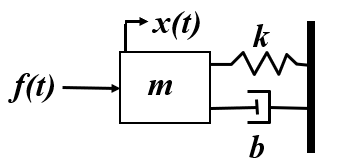
\includegraphics[width=0.3\textwidth]{mass-spring.png}
\end{center}
\[\sum F= m\ddot{x} \quad \implies \quad  m\ddot{x}+ b\dot{x} + kx = f(t)\]
The state variables can be defined as position $x$ and velocity $\dot{x}$.\\\\
Generally, \hl{linear time-invariant (LTI) systems} can be represented by an $n^{th}$ order linear differential equation of the form:
\[a_n y^{(n)} + a_{n-1} y^{(n-1)} + \cdots + a_1 \dot{y} + a_0 y = b_m u^{(m)} + b_{m-1} u^{(m-1)} + \cdots + b_1 \dot{u} + b_0 u\]
Where $u(t)$ is the input and $y(t)$ is the output of the system.\\\\
A LTI system is \hl{linear} if it satisfies the superposition principle, and \hl{time-invariant} if its coefficients do not change with time.
\newpage
\underline{For example}:
\begin{itemize}
    \item $\ddot{x} + 3t\dot{x} + 2x = 0$  is linear but not time-invariant
    \item $\ddot{x} + 3\dot{x} + 2x = 0$ is linear and time-invariant
    \item $\ddot{x} + 3\dot{x}+ 2x^2 = 0$ is nonlinear and time-invariant
\end{itemize}
\section*{Linear and Nonlinear Systems}
As mentioned before, linear systems obey superposition. This is especially useful when analyzing the response of a system subjected to multiple inputs. In that case, the response of the system to each input can be analyzed separately and then summed to find the total response.\\\\
Nonlinear systems involve nonlinear relationships among their state variables and inputs, such as exponentials, products, or transcendental functions, resulting in a violation of the superposition principle.\\\\
\underline{For example}: the string-mass pendulum is a nonlinear system
\begin{center}
    \includegraphics[width=0.5\textwidth]{pendulum.png}
\end{center}
Summing torques about the pivot point gives:
\[\sum \tau = I\ddot{\theta} \quad \implies \quad m\ell^2 \ddot{\theta} = -mg\ell\sin(\theta)+u(t)\]
Since there is a sinusoidal relationship to the state variable $\theta$, this system is nonlinear. However, we will see in a later section that we can linearize this system about an equilibrium.
\section*{State Space Representation}
(From ESC-251 Systems Engineering) We are able to rewrite the equations of motion of a system in the time domain into a matrix form using state variables. This is useful because it allows us to write an $n^{th}$ order system as a system of n first order equations.\\\\
The state space representation of a system is given by the following form:
\[\begin{aligned}
\dot{\underline{x}} &= [A]{\underline{x}} + [B]\underline{u} \\
\underline{y} &= [C]{\underline{x}} + [D]\underline{u}
\end{aligned}\]
\newpage
Where:
\begin{multicols}{2}
\begin{itemize}
    \item $\underline{x}$ = state vector
    \item $\underline{u}$ = input vector
    \item $\underline{y}$ = output vector
    \newcolumn
    \item $[A]$ = state matrix
    \item $[B]$ = input matrix
    \item $[C]$ = output matrix
    \item $[D]$ = direct transition matrix (output related to input)
\end{itemize}
\end{multicols}
The \hl{state vector} is a column vector that contains the state variables of the system.\\\\
Starting from the equations of motion, define state variables such that we can rewrite the equations of motion as first order differential equations. In other words, \hl{"kill the dots" (get rid of higher order derivatives) by introducing a new state variable for each derivative}.\\\\
\underline{For example}: recall the equation of motion for a mass-spring-damper system:
\[m\ddot{x}+ b\dot{x} + kx = f(t)\]
Define the state variables as:
\[x = x,\quad v=\dot{x}\]
Then we can rewrite the equation of motion as a system of first order differential equations:
\[m\dot{v}+ bv + kx = f(t)\]
\begin{eqnarray*}
\dot{x} &=& v \\
\dot{v} &=& -\frac{k}{m}x - \frac{b}{m}v + \frac{1}{m}f(t)
\end{eqnarray*}
In state space form, we can write:
\[
\underbrace{
\begin{bmatrix}
\dot{x}\\
\dot{v}
\end{bmatrix}
}_{\dot{\underline{x}}}
=
\underbrace{
\begin{bmatrix}
0 & 1\\
-\frac{k}{m} & -\frac{b}{m}
\end{bmatrix}
}_{[A]}
\underbrace{
\begin{bmatrix}
x\\
v
\end{bmatrix}
}_{\underline{x}}
+
\underbrace{
\begin{bmatrix}
0\\
\frac{1}{m}
\end{bmatrix}
}_{[B]}
\underbrace{f(t)}_{\underline{u}}
\]

\[
\underbrace{y}_{\underline{y}}
=
\underbrace{
\begin{bmatrix}
1 & 0
\end{bmatrix}
}_{[C]}
\underbrace{
\begin{bmatrix}
x\\
v
\end{bmatrix}
}_{\underline{x}}
+
\underbrace{0}_{[D]}
\underbrace{f(t)}_{\underline{u}}
\]
Check that the matrix multiplication (dot product between rows and columns) correctly reproduces the rewritten equations of motion and that the dimensions are consistent.\\\\
The output matrix is often either a matrix that selects certain state variables as outputs, or a matrix that operates on the state variables to produce the output (ie. momentum is a velocity state variable multiplied by mass). The direct transmission matrix is often zero, but it can be non-zero if the output is directly related to the input (ie. if we want to output/read the input voltage in an electrical system).
\section*{Linearization of Nonlinear Systems}
The intuition for linearization is the as from ESC-251 Systems Engineering: Generally, we do this by approximating the \textit{local} behavior of a non-linear system around an equilibrium point (operating point) using the first order Taylor expansion.\\\\
Defining the operating point as $\bar{x}$ and the incremental variable as $\hat{x}$, we can see graphically how the linearization process works:
\[\boxed{x=\bar{x}+\hat{x},\quad f(\hat{x}) = f(x)-f(\bar{x})}\]
\begin{center}
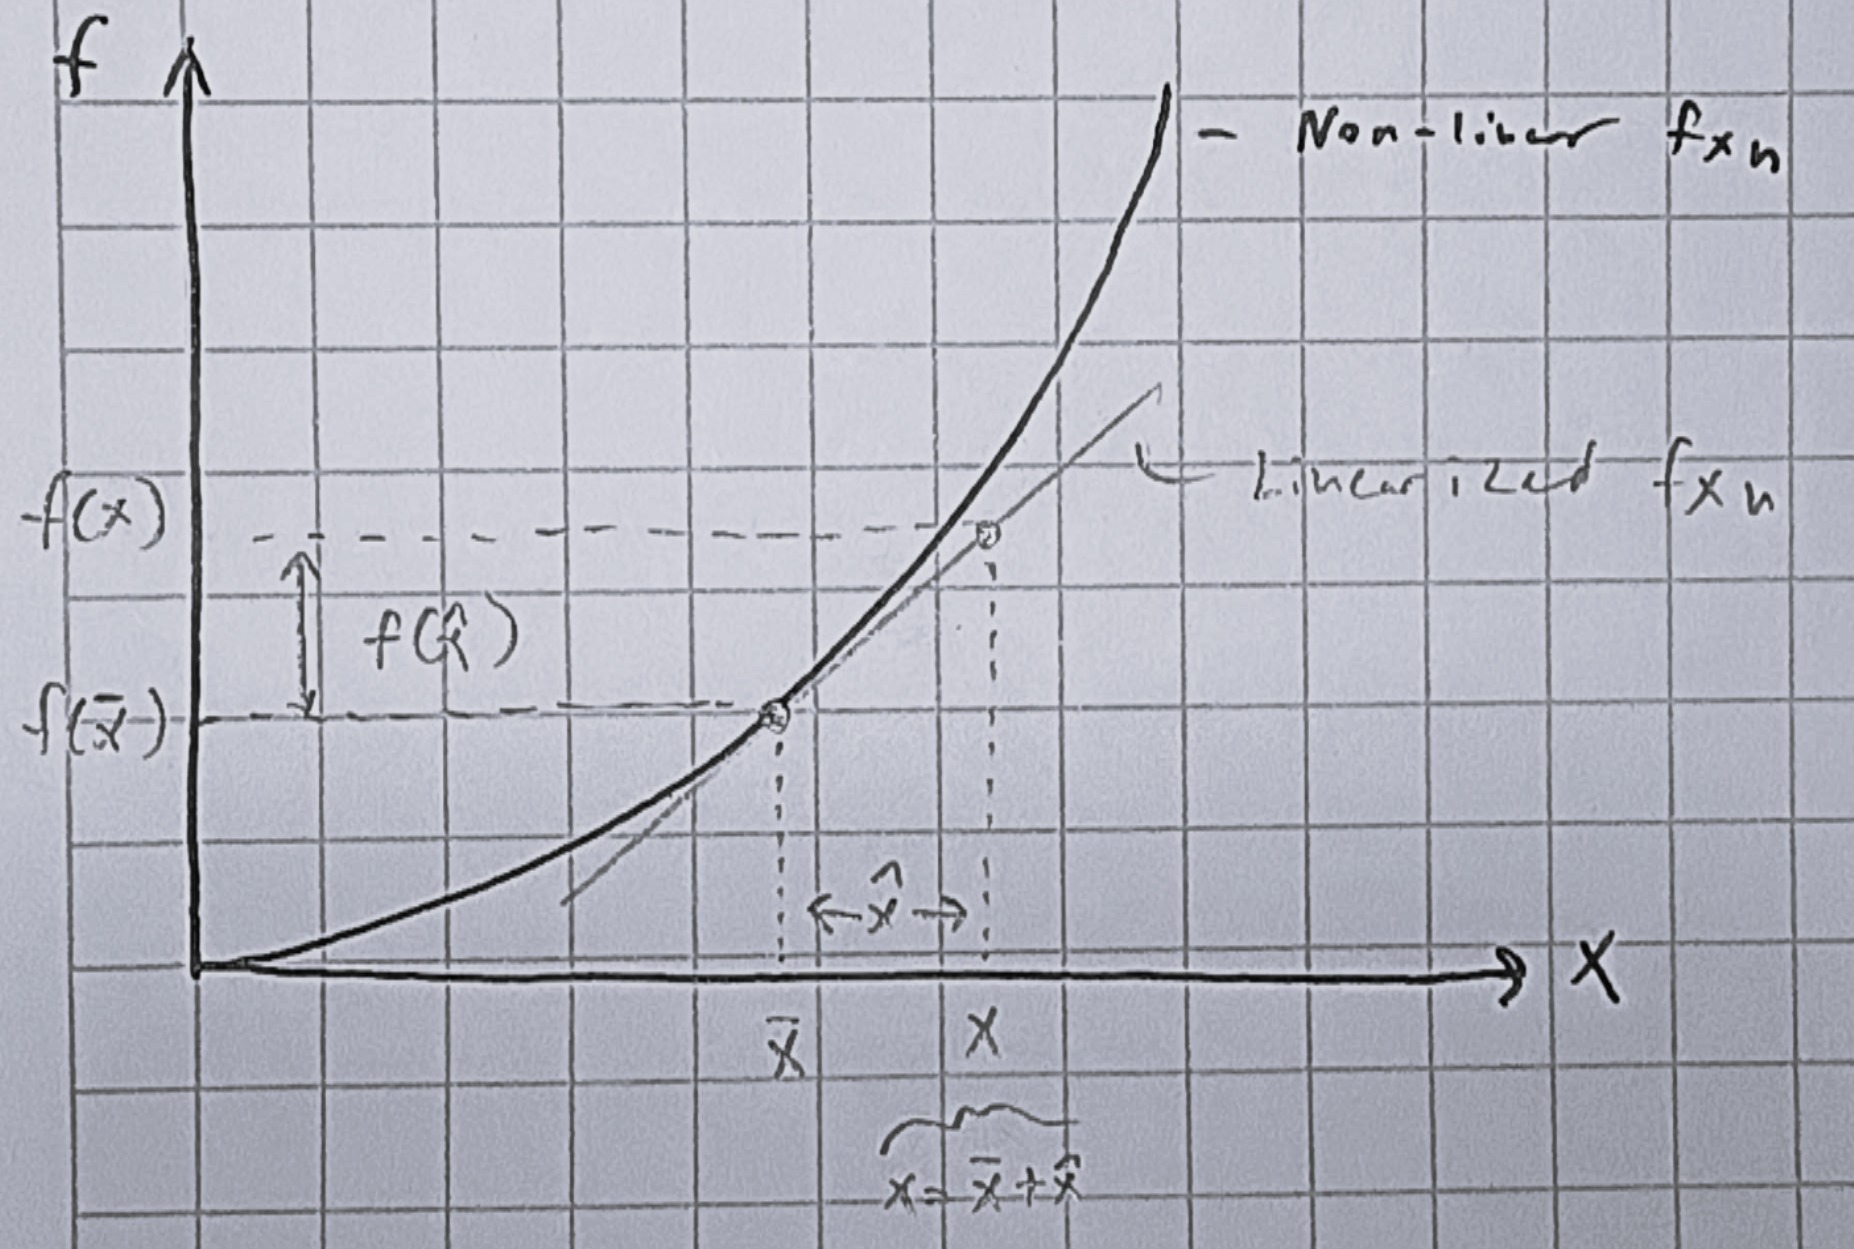
\includegraphics[width=0.7\textwidth]{Linearization.jpg}
\end{center}
Mathematically, approximating the non-linear function $f(x)$ around the operating point $\bar{x}$ gives us a tangent line that approximates the behavior of the system near $\bar{x}$:
\[k=\frac{df}{dx}\bigg|_{x=\bar{x}}\]
\[f(x) = f(\bar{x})+k(x-\bar{x})\]
Using the definition of $\hat{x}$, we can rewrite the linearized function in terms of the incremental variable $\hat{x}$:
\[f(x)=f(\bar{x})+k\hat{x}\quad \implies \quad \boxed{f(\hat{x})=k\hat{x}}\]
Now we are able to apply our techniques for linear systems to anaylze the behavior of the system under $\hat{x}$, however we must remember that the \textit{total} response of the system is given by
\[f(x) = f(\bar{x}) + f(\hat{x}),\quad x = \bar{x} + \hat{x} \]
Effectively, this linearization technique is like a transformation from the original $(x, f(x))$ coordinate system to a new $(\hat{x}, f(\hat{x}))$ coordinate system that is centered around the operating point $(\bar{x}, f(\bar{x}))$. So we need to remember to transform the results back to the original coordinate system when necessary.\\\\
\underline{Note:} The \hl{operating point is defined as the equilibrium point of the system} since the further away from the operating point we are, the worse the linear approximation will be.
\section*{Linearization Procedure}
\begin{itemize}
    \item[I.] \textbf{Define operating point \& incremental variables:} \\
    Let $f(x)$ be a non-linear function of $x$, let $\bar{x}$ be the nominal operating point and let $\hat{x} = x - \bar{x}$ be the deviation from the operating point. Linearize $f(x)$ using Taylor series or graphical method.
    
    \item[II.] \textbf{Find operating point:} \\
    To find the operating point, find the "equilibrium" solution of the system when \\$\bar{x} = (\text{constant})$ by setting $\dot{x} = \ddot{x}=0$.
    
    \item[III.] \textbf{Replace with linearized terms:} \\
    Replace the linearized $f(x)$ and $x = \hat{x} + \bar{x}$ (and $u = \hat{u} + \bar{u}$ if needed) in the non-linear differential equation.
\end{itemize}
The linearized equation is in terms of $\hat{x}$ (and $\hat{u}$ if it exists). This linearized equation describes the actual non-linear system close to the operating point. The further from the operating point, the less accurate the description is.\\\\
\underline{For example:} \textbf{Non-linear spring-mass-damper system}\\
Where the spring force is non-linear and given by $f(x) = ax^3$:
\begin{center}
    \makebox[\textwidth][c]{%
        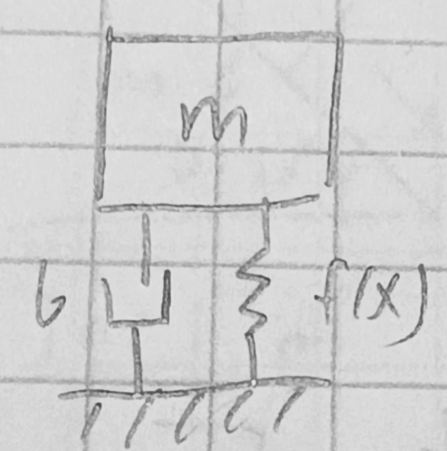
\includegraphics[width=0.25\textwidth]{nl spring 1.png}
        \hspace{0.02\textwidth}
        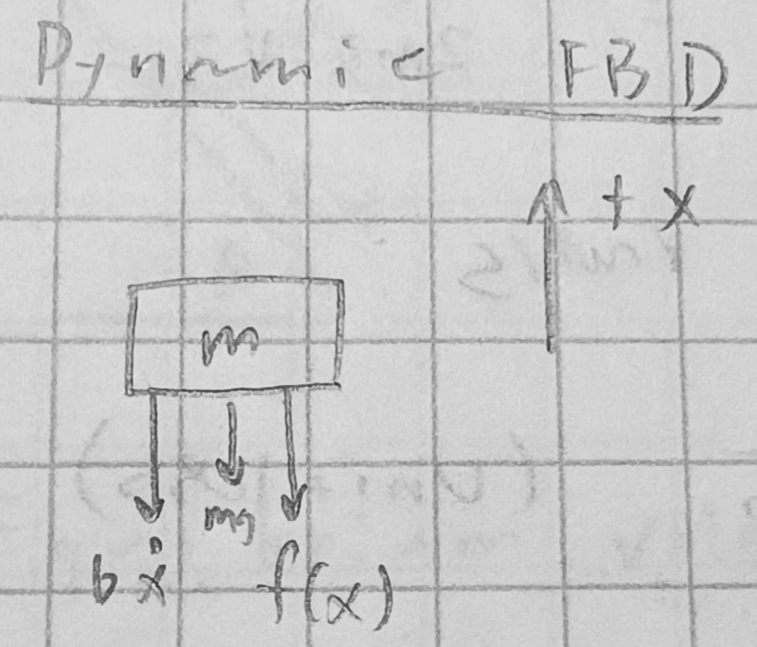
\includegraphics[width=0.3\textwidth]{nl spring 2.png}%
    }
\end{center}
The equation of motion is given by:
\[\sum F = m\ddot{x} \quad \implies \quad m\ddot{x} + b\dot{x}+ax^3 = -mg\]
Follow the linearization procedure to find the linearized equation of motion:
\begin{itemize}
    \item[I.] Define variables and linearize $f(x)$:
    \[x = \bar{x} + \hat{x}\]
    \begin{eqnarray*}
    f(x) &=&  f(\bar{x}) + \frac{df}{dx}\bigg|_{x=\bar{x}} (x-\bar{x})\\
    &=& a\bar{x}^3 + 3a\bar{x}^2(\hat{x})
    \end{eqnarray*}
    \item[II.] Find the operating (equilibrium) point by setting $\dot{x} = \ddot{x} = 0$:
\[a\bar{x}^3 = -mg\]
\[\implies \bar{x} = \sqrt[3]{-\frac{mg}{a}}\]
    \item[III.] Linearize the equation of motion:
    \[m\frac{d^2 (\bar{x}+\hat{x})}{dt^2} + b\frac{d(\bar{x}+\hat{x})}{dt} + (a\bar{x}^3 + 3a\bar{x}^2\hat{x}) = -mg\]
    Since $\bar{x}$ is constant, $\dot{\bar{x}} = \ddot{\bar{x}} = 0$:
    \[m\frac{d^2(\hat{x})}{dt^2} + b\frac{d(\hat{x})}{dt} + (a\bar{x}^3 + 3a\bar{x}^2\hat{x}) = -mg\]
    Substituting in the equilibrium condition $a\bar{x}^3 = -mg$:
    \[m\frac{d^2(\hat{x})}{dt^2} + b\frac{d(\hat{x})}{dt} + 3a\bar{x}^2\hat{x} = 0\]
\end{itemize}
Now we have a linearized equation of motion in terms of the incremental variable $\hat{x}$ that describes the behavior of the non-linear system near the operating point $\bar{x}$.
\subsection*{Jacobian Linearization Method}
The Jacobian linearization method is a systematic way to linearize a non-linear system with non-linear multiple state variables.\\\\
\textbf{Definition}: \hl{A Jacobian matrix is a matrix containing all first-order partial derivatives of a vector-valued function with respect to its input variables:}
\[
\underline{f}(\underline{x}) =
\begin{bmatrix}
f_1(x_1,\ldots,x_n) \\
\vdots \\
f_m(x_1,\ldots,x_n)
\end{bmatrix},
\qquad
\underline{x} =
\begin{bmatrix}
x_1 \\
\vdots \\
x_n
\end{bmatrix}
\]
\[
\frac{\partial \underline{f}}{\partial \underline{x}}
=
\begin{bmatrix}
\frac{\partial f_1}{\partial x_1} & \cdots & \frac{\partial f_1}{\partial x_n} \\
\vdots & \ddots & \vdots \\
\frac{\partial f_m}{\partial x_1} & \cdots & \frac{\partial f_m}{\partial x_n}
\end{bmatrix}
\]
\underline{Consider a general nonlinear system in state-space form:}
\[
\boxed{
\begin{aligned}
\dot{\underline{x}} &= \underline{f}(\underline{x},u)\\
\underline{y} &= \underline{h}(\underline{x},u)
\end{aligned}
}
\]
where $\underline{f}$ is a vector-valued function describing the time evolution of the state variables, and $\underline{h}$ is a function relating the state variables and inputs to the system outputs. Unlike an LTI system, these functions may contain nonlinear relationships.\\\\
\textbf{Example: Pendulum System}\\
Recall the pendulum system with equation of motion:
\[
m\ell^2\ddot{\theta}=-mg\ell\sin(\theta)+u(t)
\]
Let $\omega=\dot{\theta}$ and define the state vector:
\[
\underline{x}=
\begin{pmatrix}
\theta\\
\omega
\end{pmatrix}
\]
Then we can rewrite the system in state-space form:
\[
\underbrace{
\begin{pmatrix}
\dot{\theta}\\
\dot{\omega}
\end{pmatrix}
}_{\dot{\underline{x}}}
=
\underbrace{
\begin{pmatrix}
\omega\\
-\frac{g}{\ell}\sin(\theta)+\frac{1}{m\ell^2}u(t)
\end{pmatrix}
}_{\underline{f}(\underline{x},u)}
\]
With an output of $y=\theta$:
\[
\underbrace{\theta}_{y}
=
\underbrace{
\begin{pmatrix}
1 & 0
\end{pmatrix}
\underline{x}
}_{h(\underline{x},u)}
\]
Notice that the state equation is nonlinear due to the $\sin(\theta)$ term, while the output equation is linear.\\\\
\textbf{Linearization Procedure}
\begin{itemize}
    \item [I.] Define operating point \& incremental variables:\\
    Let $\dot{x} = \underline{f}(\underline{x},\underline{u})$ be a nonlinear system, and $(\underline{\bar{x}}, \underline{\bar{u}})$ be the operating point. Define incremental variables:
    \[\underline{\hat{x}} = \underline{x} - \underline{\bar{x}},\quad \underline{\hat{u}} = \underline{u} - \underline{\bar{u}}\]
    Linearize $\underline{f}(\underline{x},\underline{u})$ using the first order Taylor expansion, where the Jacobian matrices are evaluated at the operating point $(\underline{\bar{x}}, \underline{\bar{u}})$:
    \[\underline{f}(\underline{x},\underline{u}) \approx \underline{f}(\underline{\bar{x}}, \underline{\bar{u}}) + \frac{\partial \underline{f}}{\partial \underline{x}}\bigg|_{(\underline{\bar{x}}, \underline{\bar{u}})} \underline{\hat{x}} + \frac{\partial \underline{f}}{\partial u}\bigg|_{(\underline{\bar{x}}, \underline{\bar{u}})} \underline{\hat{u}}\]
    \item [II.] Find operating point:\\
    To find the operating point, solve for the equilibrium of the system when $\underline{\bar{x}}$ is constant by setting $\dot{\underline{\bar{x}}} = \underline{f}(\underline{x},\underline{u}) = 0$.
    \item [III.] Replace with linearized terms:\\
    Substitute the linearized $\underline{f}(\underline{x},\underline{u})$ and incremental variables into the nonlinear state space equations. Applying the equilibrium condition $\underline{f}(\underline{\bar{x}}, \underline{\bar{u}}) = 0$ gives the linearized state space equations:
    \[\dot{\underline{\hat{x}}} = A \underline{\hat{x}} + B \underline{\hat{u}}\]
    Where
    \[A = \frac{\partial \underline{f}}{\partial \underline{x}}\bigg|_{(\underline{\bar{x}}, \underline{\bar{u}})}, \quad B = \frac{\partial \underline{f}}{\partial \underline{u}}\bigg|_{(\underline{\bar{x}}, \underline{\bar{u}})}\]
    We can similarly linearize the output equation $\underline{y} = \underline{h}(\underline{x},\underline{u})$ with respect to the incremental variable $\underline{\hat{y}} = \underline{y} - \underline{\bar{y}}$:
    \[\underline{\hat{y}} = C \underline{\hat{x}} + D \underline{\hat{u}}\]
    Where
    \[C = \frac{\partial \underline{h}}{\partial \underline{x}}\bigg|_{(\underline{\bar{x}}, \underline{\bar{u}})}, \quad D = \frac{\partial \underline{h}}{\partial \underline{u}}\bigg|_{(\underline{\bar{x}}, \underline{\bar{u}})}\]
\end{itemize}
\textbf{Example: Pendulum System on Steroids}\\
\section*{Laplace Transforms}
\section*{Transfer Function Representation}
\subsection*{Transfer Function Matrices}
Like how we can derive transfer functions in the Laplace domain from the equations of motion, we can do the same in state space representation using matrix arithmetic. Starting with:
\[\begin{aligned}
\dot{\underline{x}} &= [A]{\underline{x}} + [B]\underline{u} \\
\underline{y} &= [C]{\underline{x}} + [D]\underline{u}
\end{aligned}\]
Taking the Laplace transform:
\[\begin{aligned}
    s\underline{X} &= [A]\underline{X} + [B]\underline{U} \\
     \underline{Y} &= [C]\underline{X} + [D]\underline{U}
\end{aligned}\]
Isolate the State Vector ($\underline{X}$):
\[\underline{X} = [sI - A]^{-1}[B]\underline{U}\]
Substitute $\underline{X}$ into the Output Equation:
\[\underline{Y} = [C]\underbrace{\left( [sI - A]^{-1}[B]\underline{U} \right)}_{\text{Sub for } \underline{X}} + [D]\underline{U}\]
Factor out $\underline{U}$ for the Transfer Function:
\[\boxed{\frac{\underline{Y}}{\underline{U}} = [C][sI - A]^{-1}[B] + [D]}\]
\underline{Recall:} We can invert a 2x2 matrix using the formula:
\[
A =
\begin{pmatrix}
a & b \\
c & d
\end{pmatrix}\]
\[A^{-1} = \frac{1}{ad - bc}
\begin{pmatrix}
d & -b \\
-c & a
\end{pmatrix},
\quad \text{if } ad - bc \neq 0.\]

\section*{Block Diagrams and System Interconnections}
\begin{center}
    {\LARGE\bfseries \fbox{System Behavior and Feedback Control}\par}
\end{center}
\section*{Poles and Zeros of Transfer Functions}
\section*{System Stability}
\section*{First- and Second-Order System Responses}
\begin{itemize}
    \item Step Response
    \item Impulse Response
    \item Frequency Response
\end{itemize}
\section*{Time Domain Specifications}
\section*{Initial/Final Value Theorems}
\section*{DC Gain and Steady-State Error}
\section*{Feedback Control and Closed-Loop Transfer Functions}
\section*{PID Controllers}
\section*{Root Locus Plots}
\begin{center}
    {\LARGE\bfseries \fbox{Frequency Response Analysis (Bode Plots)}\par}
\end{center}
\end{document}
